\definsection{Definition XV}

\begin{defin}
A circle is a plane figure contained by one line such that all the straight lines falling upon it from one point among those lying within the figure are equal to one another;
\end{defin}

In the pursuit of geometric clarity, Euclid presents us with a profound yet simple construction: the circle. Yet, it is within Definition 15 that we embark on a deeper exploration, delving into the subtleties of circle boundaries. A circle, as posited by Euclid, is not merely a figure but a boundary—the locus of all points equidistant from a given point, termed the center. This definition, while straightforward, belies a complex understanding of space and distance.

\sidenote{\raggedbottom\raggedright\ssmall{\textbf{Radius}: The distance from the center of a circle to any point on its boundary. }}
\sidenote[12][1.2cm]{\raggedbottom\raggedright\ssmall{\textbf{Diameter}: A straight line passing through the center of a circle that connects two points on its boundary.}}
\sidenote[13][2.5cm]{\raggedbottom\raggedright\ssmall{\textbf{Circumference}: The perimeter or total distance around the outer boundary of a circle.}}
\begin{figure}[h]
\centering
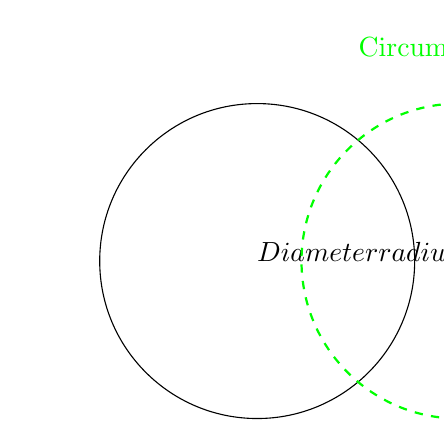
\begin{tikzpicture}
\coordinate (O) at (0,0);
\draw (O) circle (2);
\coordinate(A) at (50:2);
\coordinate(C) at (0:2);
\coordinate(B) at (180:2);
\tkzDrawSegments[blue](B,C)
\tkzDrawSegment[red](O,A)
\tkzLabelSegment[above left, blue](B,C){$Diameter$}
\tkzLabelSegment[above, sloped, red](O,A){$radius$}
\tkzLabelPoints[below](O)
 % Modifying the circumference representation
    \draw[->>,>=stealth,thick,dashed,green] (2,0) arc (0:330:2);
    % Adding curved label for the circumference
    \path (2,0) arc (0:165:2.5) node[pos=0.5,above,green] {Circumference};
\end{tikzpicture}
\caption{A Circle}
\end{figure}

Euclid's circle transcends its own simplicity, serving as a foundational element in the construction of geometric reality. It represents unity, perfection, and the infinite, embodying the philosophical underpinnings of geometry itself. 

\clearpage

The circle's boundary, or circumference, becomes a powerful tool in the exploration of the geometric universe, acting as a mediator between the finite and the infinite.

The circle's inherent properties—such as the equality of radii, the significance of the diameter, and the concept of the circle as a perfect figure—reflect a deeper metaphysical order. Through Euclid's lens, the circle is not just a figure but a manifestation of geometric harmony, embodying principles that are both mathematical and philosophical.